\documentclass[letterpaper,10pt]{article}

\usepackage{titling}
\usepackage{listings}
\usepackage{url}
\usepackage{setspace}
\usepackage{subfig}
\usepackage{sectsty}
\usepackage{pdfpages}
\usepackage{colortbl}
\usepackage{multirow}
\usepackage{relsize}
\usepackage{amsmath}
\usepackage{fancyvrb}
\usepackage{amsmath,amssymb,amsthm,graphicx,xspace}
\usepackage[titlenotnumbered,noend,noline]{algorithm2e}
\usepackage[compact]{titlesec}
\usepackage{paratype} 
\usepackage[T1]{fontenc}
\usepackage{tikz}
\usetikzlibrary{arrows,automata,shapes,trees,matrix,chains,scopes,positioning,calc}
\tikzstyle{block} = [rectangle, draw, fill=blue!20, 
    text width=2.5em, text centered, rounded corners, minimum height=2em]
\tikzstyle{bw} = [rectangle, draw, fill=blue!20, 
    text width=4em, text centered, rounded corners, minimum height=2em]

\definecolor{namerow}{cmyk}{.40,.40,.40,.40}
\definecolor{namecol}{cmyk}{.40,.40,.40,.40}

\let\LaTeXtitle\title
\renewcommand{\title}[1]{\LaTeXtitle{\textsf{#1}}}


\newcommand{\handout}[5]{
  \noindent
  \begin{center}
  \framebox{
    \vbox{
      \hbox to 5.78in { {\bf ECE254: Operating Systems and Systems Programming } \hfill #2 }
      \vspace{4mm}
      \hbox to 5.78in { {\Large \hfill #4  \hfill} }
      \vspace{2mm}
      \hbox to 5.78in { {\em #3 \hfill} }
    }
  }
  \end{center}
  \vspace*{4mm}
}

\newcommand{\lecture}[3]{\handout{#1}{#2}{#3}{Lecture #1}}
\newcommand{\tuple}[1]{\ensuremath{\left\langle #1 \right\rangle}\xspace}

\addtolength{\oddsidemargin}{-1.000in}
\addtolength{\evensidemargin}{-0.500in}
\addtolength{\textwidth}{2.0in}
\addtolength{\topmargin}{-1.000in}
\addtolength{\textheight}{1.75in}
\addtolength{\parskip}{\baselineskip}
\setlength{\parindent}{0in}
\renewcommand{\baselinestretch}{1.5}
\newcommand{\term}{Spring 2015}

\singlespace


\begin{document}

\lecture{ 16 --- Deadlock Avoidance}{\term}{Jeff Zarnett}

\section*{Dealing with Deadlock, Continued}
Continuing from before, there were four techniques for how to deal with deadlock and we examined the first two. Now we proceed by examining the third: deadlock avoidance.

\subsection*{Deadlock Option 3: Deadlock Avoidance}
In examining deadlock prevention, we were attempting to rule deadlock out categorically by eliminating one of the three preconditions for deadlock to be possible. If successful, then we can be sure that deadlock does not occur. Unfortunately, eliminating the pillars came with some conditions and the best we could accomplish was merely making deadlock less likely and not resolving the problem in its entirety. Thus, we are forced to live with a system where a deadlock is possible. However, deadlock being possible is not the same thing as deadlock being inevitable; we can take steps to avoid it if there is a danger of it actually happening. The basic strategy is: do not allow a cycle in the resource allocation graph.

In the dining philosophers problem, one strategy to prevent the deadlock was limiting the number of concurrently-eating philosophers to four, even though the table has five seats. This was a way of preventing a cycle in the resource allocation graph: with only four philosophers and five forks, there were insufficient requests to complete a cycle. This solution is suitable, but not necessarily generalizable to all deadlock situations.

\subsubsection*{Ordering of Resources}
A general strategy to prevent a cycle from forming is to impose ordering on resource requests. Resources are given some order and requests must follow that order. This idea may have occurred seemed obvious from this example: 

\begin{multicols}{2}
\textbf{Thread P}\vspace{-2em}
  \begin{verbatim}
	 1. wait( a ) 
	 2. wait( b )
	 3. [critical section]
	 4. signal( a )
	 5. signal( b )
  \end{verbatim}
\columnbreak
\textbf{Thread Q}\vspace{-2em}
  \begin{verbatim}
	 1. wait( b ) 
	 2. wait( a )
	 3. [critical section]
	 4. signal( b )
	 5. signal( a )
  \end{verbatim}
\end{multicols}
\vspace{-2em}

Thread $Q$ requests \texttt{b} first and then \texttt{a}, while $P$ does the reverse. The deadlock would not take place if both threads requested these two resources in the same order, whether \texttt{a} then \texttt{b} or \texttt{b} then \texttt{a}. Of course, when they have names like this, a natural ordering (alphabetical, or perhaps reverse alphabetical) is obvious. 

To generalize and formalize this principle, if the set of all resources in the system is $R = \{R_{0}, R_{1}, R_{2}, ... R_{m}\}$, we assign to each resource $R_{k}$ a unique integer value. Let us define this function as $f(R_{i})$, that maps a resource to an integer value. This integer value is used to compare two resources: if a process has been assigned resource $R_{i}$, that process may request $R_{j}$ only if $f(R_{j}) > f(R_{i})$. Note that this is a strictly greater-than relationship; if the process needs more than one of $R_{i}$ then the request for all of these must be made at once (in a single request). To get $R_{i}$ when already in possession of a resource $R_{j}$ where $f(R_{j}) > f(R_{i})$, the process must release any resources $R_{k}$ where $f(R_{k}) \geq f(R_{i})$. If these two protocols are followed, then a circular-wait condition cannot hold~\cite{osc}.

In the dining philosophers problem, we assign each of the five chopsticks a number from 0 to 5. Each philosopher must then request them in ascending order. The first philosopher requests chopstick 0, on her left, and then chopstick 1, on her right. The second requests chopstick 1 and then chopstick 2. This continues until the last philosopher who would previously have requested chopstick 4 and then 0, but under the new rules, this is forbidden. This philosopher must instead request 0 on his right, and then 4, on his left. This last philosopher will be blocked when trying to acquire chopstick 0 and it means chopstick 4 will be available for the second-to-last philosopher. Thus, deadlock is avoided.

In~\cite{osc} is a proof that ordering the resources prevents deadlock. The approach is proof by contradiction: assume a circular wait is present. Let the set of processes in the circular wait be $\{P_{0}, P_{1}, ... P_{n}\}$ and the set of resources be $\{R_{0}, R_{1}, ... R_{n}$. The cycle is formed as: $P_{i}$ is waiting for resource $R_{i}$ and that resource is held by $P_{i+1}$. The exception is the case of $P_{n}$, which is waiting for resource $R_{n}$ that is held by $P_{0}$ (completing the cycle by wrapping around). Since Process $P_{i+1}$ holds resource $R_{i}$ while requesting $R_{i+1}$, this means $f(R_{i}) < f(R_{i+1})$ for all $i$. But this means that $f(R_{0}) < f(R_{1}) < ... < f(R_{n}) < f(R_{0})$. It cannot be the case that $f(R_{0}) < f(R_{0})$: a contradiction, meaning a circular wait cannot occur.

Enforcement of the protocol may be the responsibility of the application developers or the operating system. If the latter, we can be certain that there is no cycle; if the former, then we have once again only reduced the likelihood that deadlock exists. 

\subsubsection*{Stay Alert Stay Safe\footnote{If this reference makes no sense to you, it's because I'm old: https://www.youtube.com/watch?v=cgvv4wnVlFU}}

Suppose that instead of ordering the resources, each process will need to give the operating system some additional information about what resources might be requested. Processes need to say in advance of execution what is the maximum number of resources of each type they might conceivably need. In a system with a tape drive and printer, perhaps process $A$ needs the tape drive first, then the printer, and process $B$ needs the printer and then the tape drive. With this knowledge, the system can make more intelligent decisions about when to run a process or make it wait, to avoid getting into a deadlock~\cite{osc}.

Recall from earlier the joint progress diagram for threads $P$ and $Q$:

\begin{center}
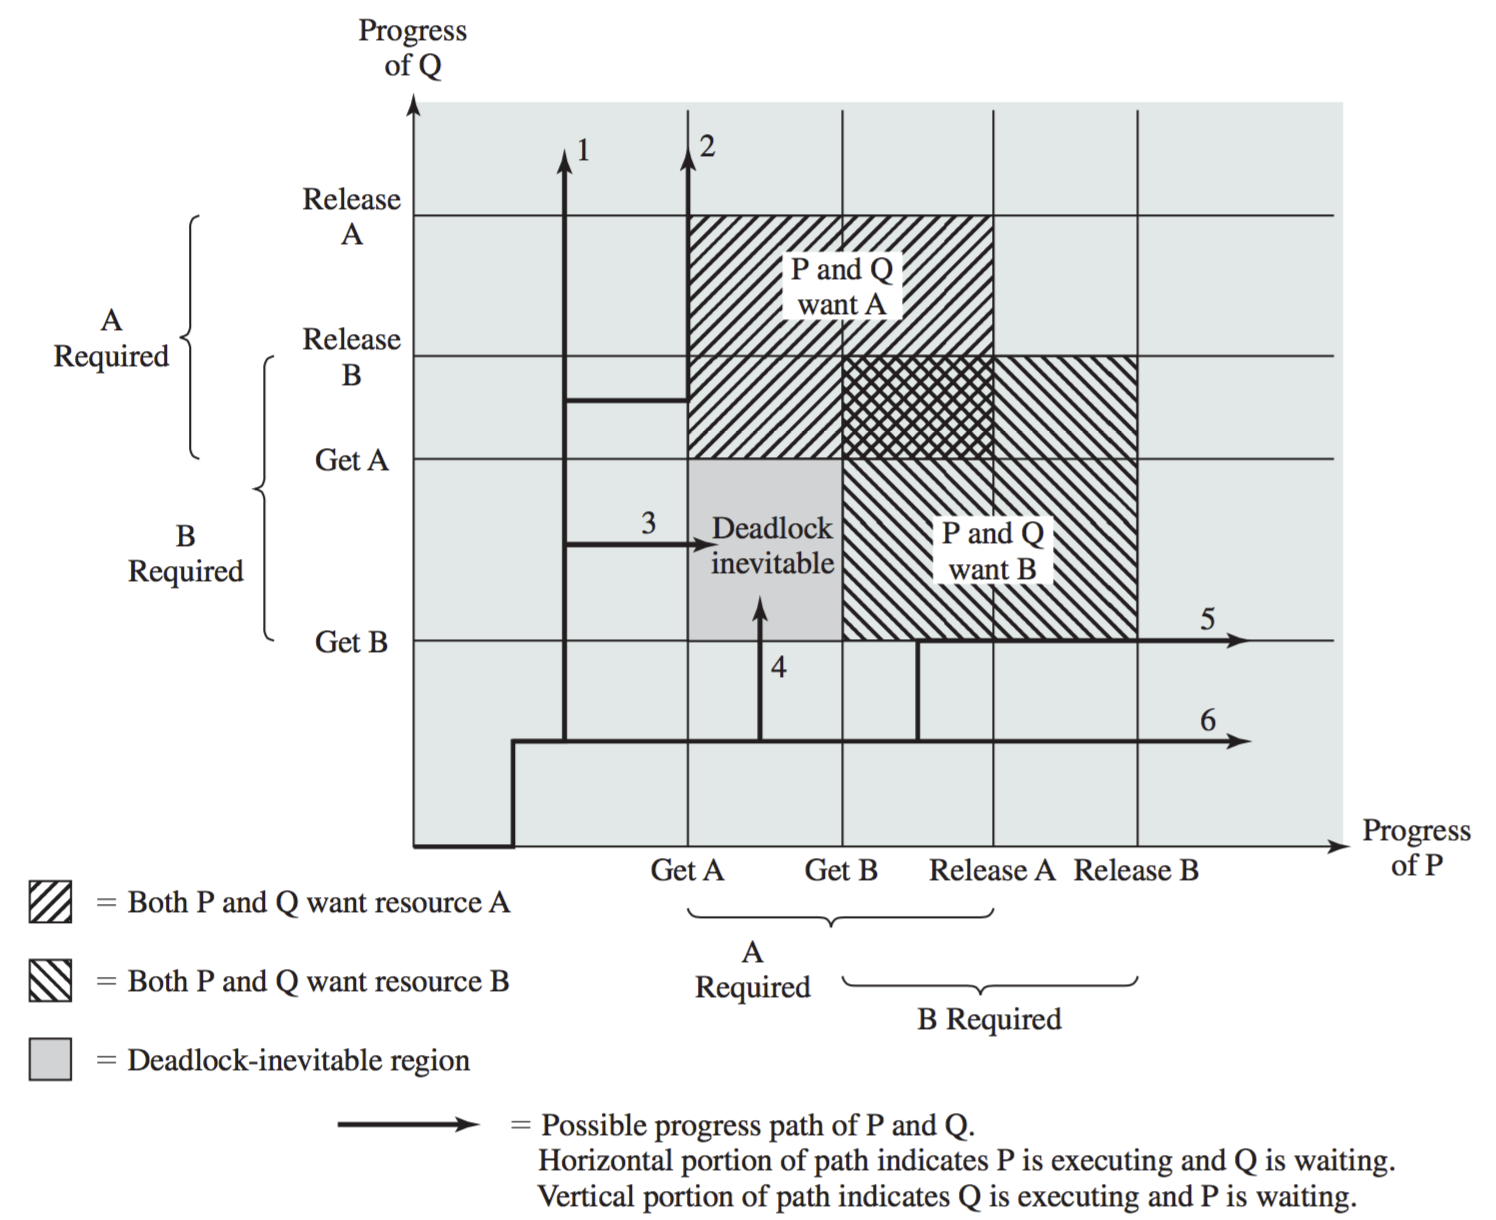
\includegraphics[width=0.75\textwidth]{images/joint-progress}\\
A joint progress diagram representing the behaviour of the $P$ and $Q$ code~\cite{osi}.
\end{center}

Every point in the diagram represents a joint state of the two processes. (e.g., $P$ wants \texttt{a} and $Q$ has it) and there are, in this example, six paths of execution, two of which will certainly result in deadlock. The other four will not.  With a single processor, all paths are horizontal or vertical (never diagonal), and the lines may only move up and right, never down or left because processes cannot run backwards in time~\cite{mos}. This diagram is the basis for analyzing the situation and deciding what to do.

We say a state is \textit{safe} if there is some scheduling order in which every process can run to completion even if all of them suddenly request their maximum resources immediately~\cite{mos}. Hence why we needed to know in advance the maximum resources that could be required by the process. 

More formally, there must exist a \textit{safe sequence}: a sequence of processes $<P_{1}, P_{2}, ... P_{n}$ is a safe sequence if the current allocation state if, for each $P_{i}$ the resource requests that $P_{i}$ can still make can be satisfied by the currently available resources plus resources held by $P_{j}$ where $j < i$. If a resource $P_{i}$ needs is not currently available, $P_{i}$ can wait until all $P_{j}$ have finished and releases its resources. When $P_{i}$ terminates, $P_{i+1}$ can obtain its needed resources and continue~\cite{osc}.

Any state that is not safe is considered \textit{unsafe}. If the system is in a safe state, then there is no deadlock. Being in an unsafe state does not mean that there is a deadlock, but it means a deadlock is possible. The analysis we do is the worst case scenario: every process immediately requests the maximum resources it could ever use. Perhaps the processes do not make those requests in reality.

Consider an example from~\cite{mos} in which there are three processes, $A$, $B$, and $C$. Assume there is only one resource, and a maximum of 10 instances exist. Suppose $A$ has 3 resources but may request up to 9, $B$ has 2 and may request up to 4, $C$ has 2 and may request up to 7. There are 3 resources currently free. How do we determine that the state described below is safe?

\begin{center}
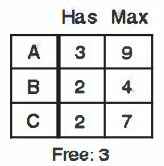
\includegraphics[width=0.15\textwidth]{images/safe-state-initial.png}\\
A diagram representing the resource allocation state of the system~\cite{mos}.
\end{center}

Recall that for a state to be safe we need only one path that allows all processes to complete. Multiple solutions may exist, and there may be paths that lead to deadlock. But we need only one solution, such as:

\begin{center}
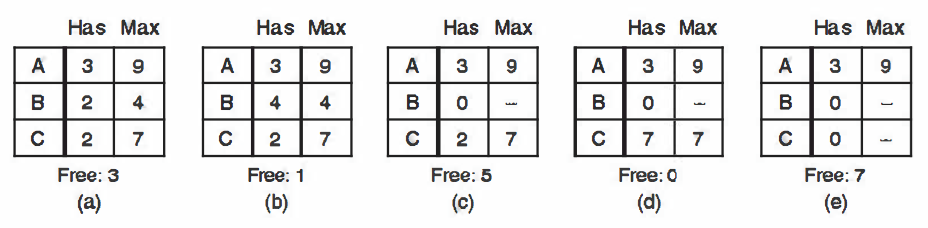
\includegraphics[width=0.75\textwidth]{images/safe-state.png}\\
A diagram demonstrating the state in (a) is safe~\cite{mos}.
\end{center}

The part of the diagram labelled (a) is the initial state of the system. Imagine that process $B$ is allowed to run exclusively, until it gets two more resources, so it now has 4 resources and there is one free, as diagram (b) depicts. $B$ is allowed to run to completion, and it therefore finishes and releases its resources to the free pool, shown in (c). Then process $C$ is scheduled and gets its full complement of resources, consuming all the elements in the free pool, as in (d). $C$ runs exclusively until completion and it releases its resources, shown in (e). Finally, $A$ is able to get all the resources and run to completion, too. Thus, we proved that the state is safe: there is a way the system can avoid a deadlock, and run all processes to completion.

Suppose, however, $A$ requests and gets another resource. In that case, the initial condition has changed so that $A$ has 4 resources and there are 2 free resources. Or, in the diagram below, the state changes from (a) to (b).

\begin{center}
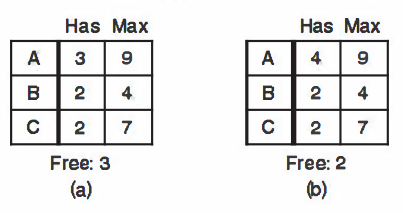
\includegraphics[width=0.35\textwidth]{images/unsafe-state-initial.png}\\
A diagram representing the updated resource allocation state of the system~\cite{mos}.
\end{center}

Given this new initial state (b), we need to evaluate if it is safe. 

\begin{center}
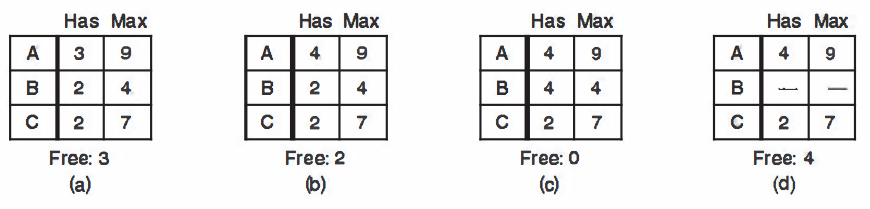
\includegraphics[width=0.70\textwidth]{images/unsafe-state.png}\\
A diagram demonstrating the state of~\cite{mos}.
\end{center}

Let us start by attempting to run $A$ - there are 3 free resources and $A$ would need 6 to continue (because a process immediately takes its full resources when it runs), so it cannot run to completion. The same is true for $C$ - it needs 5 additional resources when 3 are available. $B$, however, can continue: it needs 2 resources when 3 are available. If we attempt to run $B$ exclusively, it gets its full resources, shown in part (c), and then will terminate and release its resources, as in (d). At this point, however, there is no way to continue; neither $A$ nor $C$ can get the full complement of resources it might need because there are only 4 free resources. We are out of options; there is no path that guarantees all processes run to completion. Thus, the state is unsafe. 

Remember that just because the state is unsafe, does not mean that deadlock is present or certain. The analysis is worst-case: $C$ may never need all 7 of the resource and may run to completion with its current 2. However, in an unsafe state, we cannot be certain that deadlock will not occur.

\paragraph{Resource-Allocation-Graph Algorithm.} The fourth condition for deadlock is modelled, typically as being a resource allocation graph with a cycle in it. Idea: let us use that idea to avoid deadlock by having the operating system maintain a resource allocation graph. This is applicable if there is only one instance of each resource and requires and still requires that all the resources that a process will require must be declared in advance. However, this condition does not have to be strictly adhered to, if the system allows additional requests only when none of the process's requests have yet been made.

The model for resource allocation graphs earlier had two kinds of edges: one representing requests (a process requests a resource) and one representing allocation (a resource currently belongs to a process). We will require a new type of edge in the graph: a \textit{claim} edge, as a way of indicating a process may request a resource at some time in the future, and it is drawn with a dashed line. When the process actually makes the request for the resource, a claim edge is converted to a request edge, and upon release the assignment edge reverts to a claim edge~\cite{osc}.

\begin{center}
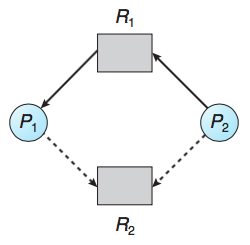
\includegraphics[width=0.25\textwidth]{images/resource-allocation-graph-claim.png}\\
A resource allocation graph showing claim edges~\cite{osc}.
\end{center}

A resource request will only be granted if converting the request edge to an assignment edge will not result in a cycle in the graph. There are graph algorithms in code that can be used to detect a cycle (and you may have studied them in a data structures and algorithms class). If no cycle is found, then allocation of the resource will not move the system into an unsafe state. If a cycle is found, the request should not be granted, as it risks a deadlock.

As mentioned, this is applicable only if all resource requests are known in advance and there is only one instance of each resource.

\paragraph{The Banker's Algorithm.} The banker's algorithm is more general: it allows for resources with multiple instances. It received this name because it is hypothetically an algorithm that a small town banker might follow if he or she were trying to prevent allocating the cash on hand in such away that he or she could no longer satisfy customers\footnote{Although the financial crisis of 2008 might convince you that the banker's algorithm is ``do whatever makes you rich and when you run out of money, the government will bail you out'', this is not the algorithm we are studying here.}. Banks typically lend out more money than they have on hand on the (usually-correct) theory that not everyone will come asking for all their deposits all at once\footnote{Not to digress too much to the subject of banking, but if it IS the case that everyone asks for their money all at once, this is called a ``run'' on the bank and is generally considered a disaster. Central banks step in with more money to fix this situation.}.

In fact, the analysis we did earlier to determine if a state is safe or unsafe, is the foundation of the banker's algorithm. Recall this diagram from earlier:

\begin{center}
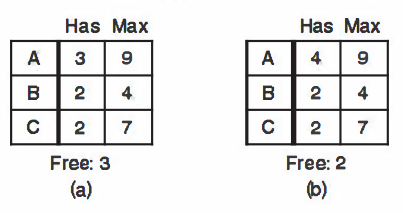
\includegraphics[width=0.35\textwidth]{images/unsafe-state-initial.png}\\
A diagram representing the updated resource allocation state of the system~\cite{mos}.
\end{center}

Granting the request from process $A$, the transition from (a) to (b), moved the system from a safe state to an unsafe state. The operating system, when it receives a resource request, will evaluate the new state to see if it would transition the system to an unsafe state. If it would result in that transition, the request will be denied or $A$ will be blocked until the request can be fulfilled without putting the system in an unsafe state. Holding to this condition means deadlock will be avoided.

The banker's algorithm can accommodate multiple resources, as shown in the diagram below.

\begin{center}
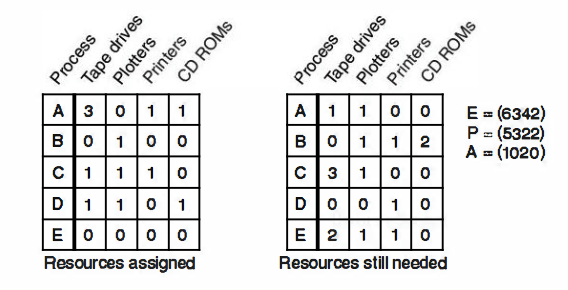
\includegraphics[width=0.6\textwidth]{images/bankers-multiple.png}\\
The banker's algorithm with multiple resources~\cite{mos}.
\end{center}

The left matrix shows the current state of assigned resources and the matrix on the right shows the maximum number of resources that a process might need to complete execution. At the far right of the diagram is a series of vectors: $E$ for the existing resources, $P$ for the resources some process currently possesses, and $A$ for the available instances of that resource.

The informal approach for checking if a state is safe is described by~\cite{mos}:
\begin{enumerate}
	\item Look for a row in the matrix, $r$, where the unmet resource needs are less than or equal to the available resources in $A$. If no such row exists, the system state is unsafe.
	\item Assume the process from $r$ gets all the resources it needs. Mark that process as terminated and put all its resources into $A$, the available pool.
	\item Repeat steps 1 and 2 until either: (i) all processes are marked terminated and the initial state was safe; or (ii) no process remains whose needs can be met and the initial state is unsafe.
\end{enumerate}

If more than one process may be chosen in step 1, it does not matter which we choose: the pool of available resources will either stay the same or get larger; it cannot shrink. 

To determine if granting a resource will make the system unsafe, the operating system should simply perform a what-if calculation. Assume the resource is granted and do the safe state calculation given that new state. If the result is that the state is unsafe, the request should be deferred or denied.

A formal, mathematical description of the banker's algorithm is defined in~\cite{osc}

As great as the banker's algorithm is in theory, in practice it is utterly useless, as highlighted by~\cite{mos}. Processes rarely know in advance what their maximum resource needs will be. Also, the number of processes is not fixed, but varies as users log in and launch and close programs and log out. Finally, a resource that was thought to be available can suddenly vanish (a peripheral device is disconnected, the network goes down, a printer breaks...). Thus in practice, the banker's algorithm can almost never be used.


\subsubsection*{Summary of Avoidance}

Avoidance techniques may be useful in preventing a deadlock from occurring without having to preempt resources or forbidding hold-and-wait conditions. Unfortunately, it requires a fixed number of known resources to allocate, and more importantly, a great deal of foreknowledge about what resources a process might need at some point in the future. Finally, because it deals with the worst case, avoidance techniques may result in denial or deferment of requests that will not actually lead to a deadlock, reducing system performance in the name of safety.

\subsubsection*{Other Recommendations}

The avoidance techniques discussed previously require perfect information (or at least, accurate worst-case guesses) about all the resources a process will ever need. In a world where this information is not known, thus far, all we have managed is to make deadlock less likely, not prevent it entirely. There are some further recommendations from~\cite{rtsda} that we should follow to make it more likely we avoid a deadlock:

\begin{enumerate}
\item Minimize the number of critical sections and their length. Mutual exclusion should be applied only where it is needed and to the minimal number of program statements.

\item All tasks must release semaphores and resources as soon as possible. This is not just polite (making other processes wait unnecessarily is just plain rude), but also makes it less likely that processes are stuck waiting for one another.

\item Do not suspend tasks when in the critical region. Avoid calling yield or some other call known to block.

\item All critical regions must be error-free. This is obviously a desirable property for the whole program, but in critical region we must be especially careful.

\item Do not allocate resources in interrupt handlers. Any resource allocation might block, and if an interrupt handler gets blocked, the whole system can be stuck.

\item Always perform validity checks on pointers (or null checks) in critical regions. A segmentation fault or exception in the critical region can also mean never releasing the lock.

\end{enumerate}




\bibliographystyle{alpha}
\bibliography{254}


\end{document}